\documentclass[tikz,border=6pt]{standalone}
\usepackage{tikz}
\begin{document}
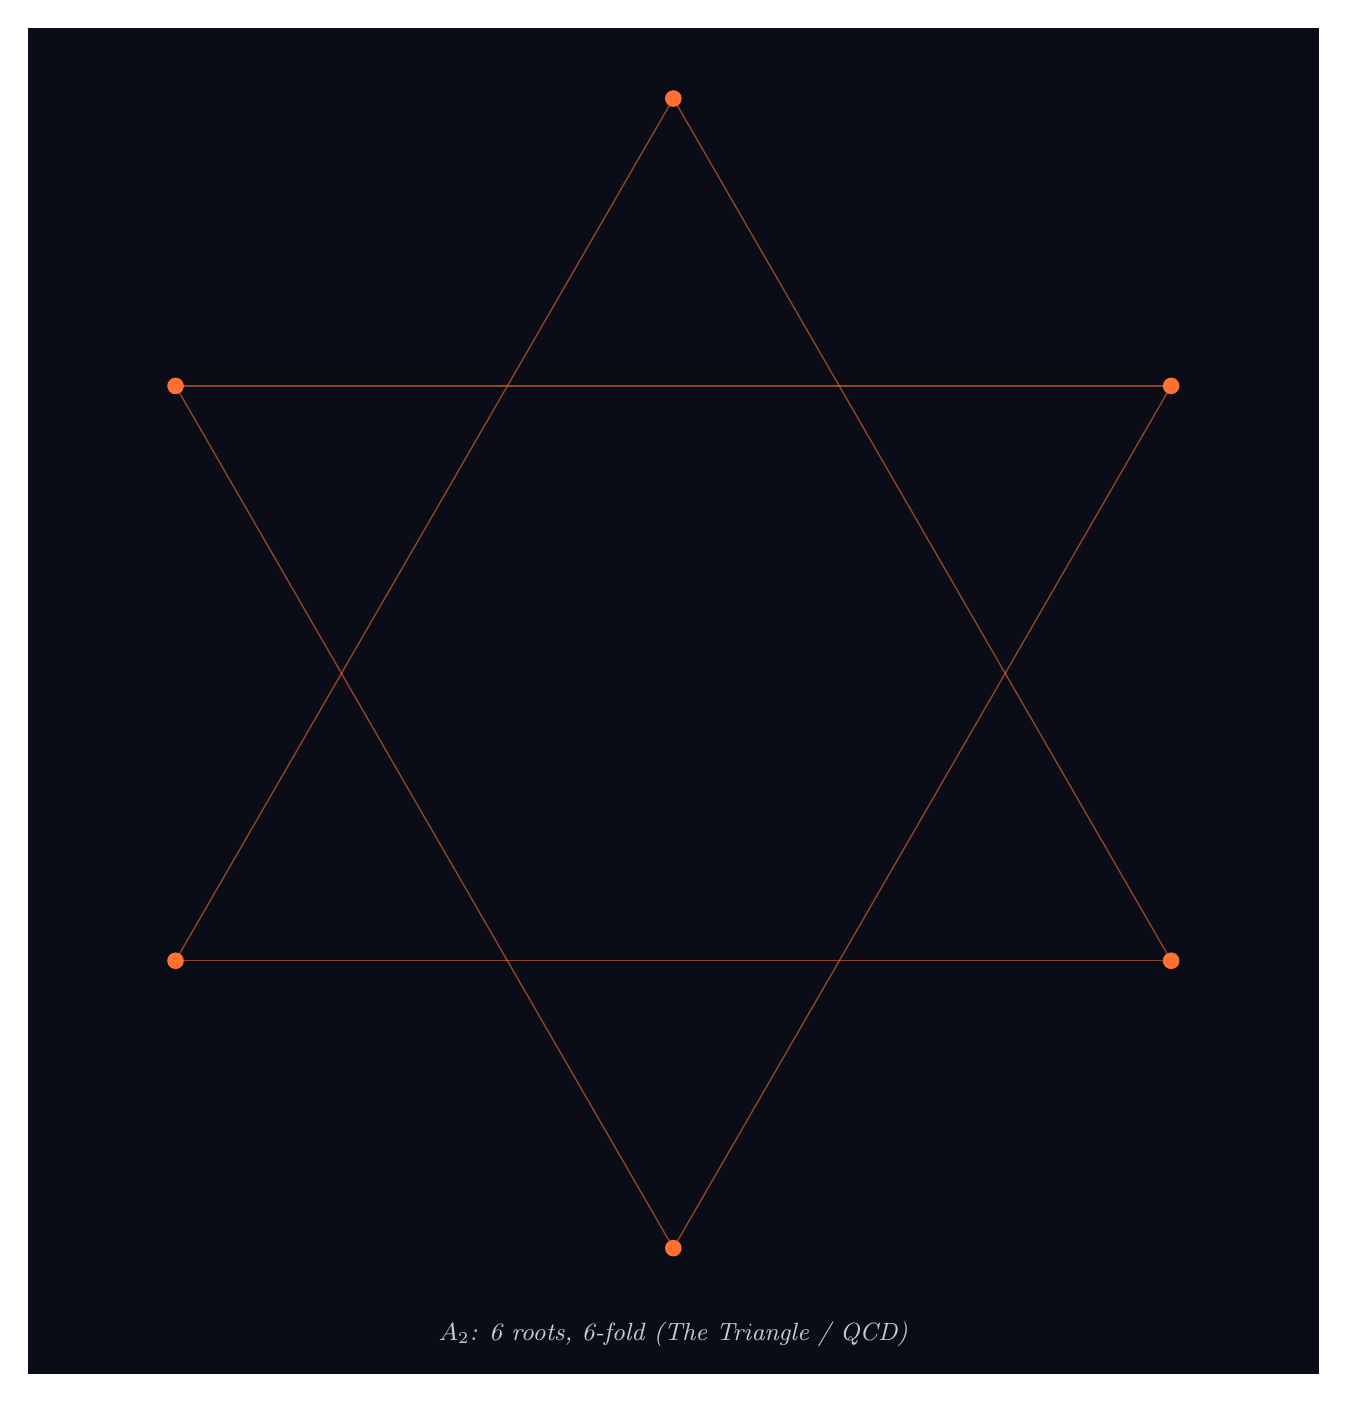
\begin{tikzpicture}
\definecolor{ring0}{rgb}{1.000,0.440,0.200}
\definecolor{bg}{rgb}{0.04,0.05,0.09}
\fill[bg] (-8.2,-8.9) rectangle (8.2,8.2);
\draw[ring0,line width=0.5pt,opacity=0.55] (-0.000,-7.300)--(-6.322,3.650);
\draw[ring0,line width=0.5pt,opacity=0.55] (-0.000,-7.300)--(6.322,3.650);
\draw[ring0,line width=0.5pt,opacity=0.55] (-6.322,3.650)--(6.322,3.650);
\draw[ring0,line width=0.5pt,opacity=0.55] (0.000,7.300)--(6.322,-3.650);
\draw[ring0,line width=0.5pt,opacity=0.55] (0.000,7.300)--(-6.322,-3.650);
\draw[ring0,line width=0.5pt,opacity=0.55] (6.322,-3.650)--(-6.322,-3.650);
\fill[ring0] (-0.000,-7.300) circle (3.0pt);
\fill[ring0] (-6.322,3.650) circle (3.0pt);
\fill[ring0] (6.322,3.650) circle (3.0pt);
\fill[ring0] (0.000,7.300) circle (3.0pt);
\fill[ring0] (6.322,-3.650) circle (3.0pt);
\fill[ring0] (-6.322,-3.650) circle (3.0pt);
\node[white!80!black,font=\small\itshape] at (0,-8.4) {$A_2$: 6 roots, 6-fold (The Triangle / QCD)};
\end{tikzpicture}
\end{document}